%=========================
\chapter{L'association}
%=========================

\begin{center}
	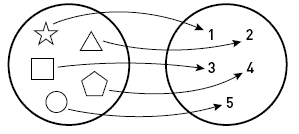
\includegraphics[width=5.66cm,height=2.536cm]{image/a2012Logique2eme-img014.png}
\end{center}
	

%=====================
\section{Introduction}
%=====================
	
	Dans ce chapitre, nous considérons des ensembles de données 
	possédant une \textbf{clé} (aussi appelée \textbf{identifiant}). 
	Par définition, la clé est unique pour chaque élément de l'ensemble. 
	Vous connaissez déjà de nombreux exemples par le cours de 
	bases de données, citons entre autres~:

	\begin{itemize}
		\item {
			le numéro d'étudiant, unique pour chaque étudiant de l'ESI}
		\item {
			le numéro de châssis d'un véhicule automobile}
		\item {
			le numéro de catalogue des produits vendus dans une grande surface}
		\item {
			le code postal des communes de Belgique, etc.}
	\end{itemize}

	Pour pouvoir stocker les éléments de ce type d'ensemble 
	dans le cadre de processus qui requièrent des accès fréquents
	aux données, nous devons recourir -- parmi les structures de 
	données vues jusqu'ici -- au tableau ou à la liste (la
	liste non chainée vue en 1\textsuperscript{ère} année). 
	L'inconvénient de ces structures réside dans le fait de devoir
	localiser les données par un indice, qui est dans la plupart 
	des cas un numéro d'ordre arbitraire qui n'est pas
	directement lié à la clé ; il faut donc toujours accompagner 
	la structure choisie d'un outil de recherche, ce qui
	implique un parcours des données pour chacune des opérations 
	de bases telles que la modification, la consultation ou la
	suppression d'un élément.

	Prenons l'exemple des étudiants de l'ESI dont l'identifiant 
	est un entier de 5 chiffres (par ex. 35421). Si on stocke
	les données dans un tableau par ordre alphabétique, il est 
	évident que l'indice de la case où se trouve un étudiant
	donné n'aura aucun rapport direct avec son numéro d'étudiant. 
	De même si on trie les données sur les numéros
	d'étudiant, rien ne permet de le localiser directement, 
	si ce n'est dans ce cas que la recherche pourrait être
	accélérée (par une recherche dichotomique par ex.). 
	On pourrait aussi envisager de placer un étudiant directement dans
	la case correspondant à son numéro d'étudiant (ainsi, l'étudiant 35421 
	serait dans la case 35421) mais ce n'est pas une
	idée très heureuse car elle exigerait d'utiliser un tableau 
	énorme dont la majorité des cases seraient inutilisées (il
	n'y a pas 35000 étudiants à l'ESI !) et de plus le tableau 
	contiendrait de nombreux trous (il n'y a pas un étudiant
	pour chacun des numéros dans un intervalle donné, certains 
	numéros disparaissent par exemple suite à un abandon).

	Nous allons dans ce chapitre construire une structure qui 
	permet de faire la liaison directe entre un élément et sa clé,
	et qui nous dispensera du problème «~technique~» de devoir 
	rechercher cet élément dans la structure. La connaissance de
	sa clé devrait permettre de le localiser immédiatement par 
	un algorithme de complexité minimale (en O(1) plutôt que en
	O(\textit{n})).


%===================
\section{Définition}
%===================

	Une \textbf{association} (on dit aussi \textit{dictionnaire} 
	ou encore \textit{map} selon la terminologie anglaise) lie
	des éléments à leur clé (ou identifiant). Il s'agit d'une 
	structure de données qui contient des couples (clé, valeur)
	et qui autorise les opérations suivantes~: stocker, retirer 
	et modifier un élément à partir de sa clé, connaitre le
	nombre d'éléments de l'ensemble (c'est-à-dire le nombre de 
	couples), et obtenir la liste des clés des éléments présents
	dans la structure.
	

%==================================
\section{Description orienté-objet}
%==================================

	Nous allons définir une classe Map (pour des raisons pratiques, 
	nous optons pour le nom anglais en raison de sa
	brièveté) dont les méthodes réalisent les opérations 
	citées ci-dessus. Les éléments contenus dans cette «~map~» sont
	des couples (clé, valeur). Plus précisément ce sont des variables 
	structurées dont les champs sont d'une part la clé
	(de type K, le plus souvent un entier ou une chaine de caractère) 
	et d'autre part la valeur (de type T quelconque). En
	particulier, la clé peut être elle-même un champ de la 
	valeur, ce qui peut paraitre redondant, mais nécessaire pour le
	fonctionnement de la classe.
	
	\cadre{
		\begin{pseudo}
			\Class{Map<K, T>}
			\LComment K est le type de la clé
			\LComment et T celui de la valeur
				\Private
					\LComment choix à détailler plus tard
				\Public 
					\ConstrSign{Map<K, T>}{...} 
					\RComment initialise la structure vide
					\MethodSign{setÉlément}{clé~: K, val~: T}{}
					\RComment ajoute le couple de clé donnée
					\MethodSign{getValeur}{clé~: K}{T}
					\RComment retourne la valeur associée à la clé
					\MethodSign{supprimer}{clé~: K}{}
					\RComment retire le couple associé à la clé
					\MethodSign{contient}{clé~: K}{booléen}
					\RComment indique si le couple de clé donnée est présent
					\MethodSign{taille}{}{entier}
					\RComment retourne le nombre de couples
					\MethodSign{listeClés}{}{Liste<K>}
					\RComment retourne la liste des clés présentes
			\EndClass
		\end{pseudo}
	}

	La méthode \textstyleCodeInsr{setÉlément} peut éventuellement 
	écraser une valeur précédente si la clé était déjà présente. 
	Les méthodes \textstyleCodeInsr{getValeur} et 
	\textstyleCodeInsr{supprimer} génèrent un message d'erreur si la clé en
	paramètre est absente de l'ensemble. La dernière méthode est 
	nécessaire pour pouvoir parcourir les éléments de l'ensemble. 
	En effet, sa structure interne étant un attribut privé inconnu 
	à l'extérieur de la classe, il est nécessaire d'avoir un outil 
	donnant la liste des clés présentes. En parcourant la liste et 
	en utilisant la méthode \textstyleCodeInsr{getValeur}, 
	on pourra ainsi passer en revue tous les éléments de l'association. 
	Il est à noter que la liste retournée n'est pas forcément dans 
	l'ordre des clés, c'est une limitation de cette structure.
	

%==============================
\section{Exemple d'utilisation}
%==============================

	Illustrons par un exemple l'utilité de la classe Map. Supposons qu'on
	veuille faire des statistiques sur les marques de voitures d'un grand 
	parc automobile. On voudrait connaitre le nombre de véhicules pour 
	chacune des marques présentes. Les données sont contenues dans un fichier 
	\textbf{fichAuto} dont chaque enregistrement de type Voiture contient 
	les champs \textbf{marque} (chaine), \textbf{modèle} (chaine),
	\textbf{immatriculation} (chaine), et d'autres données qui ne sont 
	pas utiles ici.
	
	Écrivons une première version sans utiliser la classe Map. 
	Nous avons besoin d'un compteur associé à chacune des marques de voitures. 
	Il est possible d'utiliser un tableau, mais avec l'inconvénient de ne 
	pas savoir à l'avance le nombre de marques différentes
	(ce qui pourrait se solutionner en déclarant le tableau avec une 
	taille raisonnablement grande dans ce contexte, 500 par exemple). 
	Nous allons plutôt opter pour une liste (classe Liste), 
	dont les éléments seront une structure \textbf{eltListe} 
	contenant les champs \textbf{marque} (chaine) et \textbf{cpt} (entier). 
	La démarche est simple~:
	lorsqu'une nouvelle marque est rencontrée, il faut ajouter un compteur 
	dans la liste initialisé à 1 ; si la marque a déjà été rencontrée, 
	il faut retrouver le compteur associé à cette marque et l'incrémenter. 
	Un module de recherche est donc indispensable pour le bon fonctionnement.

	\cadre{
		\begin{pseudo}
			\Module{statVoitures}{fichAuto\In~: fichier de Voiture}{}
				\Decl i, ind~: entier
				\Decl enr~: Voiture
				\Decl elt~: eltListe
				\Decl listeCpt~: Liste<eltListe>
				\Let listeCpt \Gets \K{nouveau} Liste<eltListe>( )
				\Stmt fichAuto.ouvrir( )
				\Let enr \Gets fichAuto.lire( )
				\While{NON fichAuto.EOF( )}
					\Let ind \Gets recherche(listeCpt, enr.marque)
					\If{ind = 0}
					\RComment la marque n'a pas encore été comptée
						\Let elt.marque \Gets enr.marque
						\Let elt.cpt \Gets 1
						\Stmt listeCpt.ajouter(elt)
					\Else
					\RComment la marque est présente dans la liste
						\Let elt\Gets listeCpt.get(ind)
						\Let elt.cpt \Gets elt.cpt + 1
						\Stmt listeCpt.set(ind, elt)
					\EndIf
					\Let enr \Gets fichAuto.lire( )
				\EndWhile
				\Stmt fichAuto.fermer( )
				\For{i \K{de} 1 \K{à} listeCpt.taille( )}
					\Write listeCpt.get(i).marque, listeCpt.get(i).cpt
				\EndFor
			\EndModule
		\end{pseudo}
	}
	
	\cadre{
		\begin{pseudo}
			\Module{recherche}{liste~: Liste<eltListe>, marque~: chaine}{entier}
			\LComment recherche dans la liste l'élément correspondant à la marque en paramètre
			\LComment et retourne sa position dans la liste, 0 s'il ne s'y trouve pas.
				\Decl i~: entier
				\Decl trouvé~: booléen
				\Let trouvé \Gets faux
				\Let i \Gets 0
				\While{NON trouvé ET i < liste.taille( )}
					\Let i \Gets i + 1
					\Let trouvé \Gets liste.get(i).marque = marque
				\EndWhile
				\If{trouvé}
					\Return i
				\Else 
					\Return 0
				\EndIf
			\EndModule
		\end{pseudo}
	}

	Avec la classe Map, le code se simplifie considérablement~: 
	nous sommes débarassés du module de recherche, et du souci
	de connaitre à quel endroit se trouve le compteur associé 
	à une marque donnée. Les valeurs seront ici les compteurs, et
	les clés les marques de voitures. On utilise donc une Map<chaine, entier>~:
	
	\cadre{
		\begin{pseudo}
			\Module{statVoitures}{FichAuto\In~: fichier de Voiture}{}
				\Decl enr~: Voiture
				\Decl i~: entier
				\Decl liste~: Liste<chaine>
				\Decl compteurs~: Map <chaine, entier>
				\Let compteurs \Gets \K{nouveau} Map<chaine, entier>( )
				\Stmt fichAuto.ouvrir( )
				\Let enr \Gets fichAuto.lire( )
				\While{NON fichAuto.EOF( )}
					\If{compteurs.contient(enr.marque)}
					\LComment la marque est déjà présente dans la Map
						\Stmt compteurs.setÉlément(enr.marque, compteurs.getValeur(enr.marque) + 1)
					\Else
					\LComment la marque n'est pas encore dans la Map
						\Stmt compteurs.setÉlément(enr.marque, 1)
					\EndIf
					\Let enr \Gets fichAuto.lire( )
				\EndWhile
				\Stmt fichAuto.fermer( )
				\Let liste \Gets compteurs.listeClés( )
				\For{i \K{de} 1 \K{à} liste.taille( )}
					\Write liste.get(i), compteurs.getValeur(liste.get(i))
				\EndFor
			\EndModule
		\end{pseudo}
	}
	
	
%=======================
\section{Implémentation}
%=======================

	On voit par l'exemple précédent que l'association apparait 
	de l'extérieur comme un ensemble non ordonné, une grande
	boite dans laquelle on introduit les couples (clé, valeur) 
	et de laquelle on peut les récupérer très facilement.
	Comment cela fonctionne-t-il ? Pour implémenter une association, 
	il est bien sûr possible d'utiliser les structures déjà connues~:

	\begin{itemize}
		\item {
			un tableau (trié ou non) ou une liste dont les éléments sont 
			les couples (clé, valeur) comme dans l'exemple des
			statistiques des marques de voitures}
		\item {
			une liste chainée (triée ou non)}
		\item {
			un arbre binaire ordonné sur les clés (voir chapitre sur les arbres)}
	\end{itemize}
	
	Utiliser une de ces structures comme attribut de la classe 
	reviendrait dès lors à camoufler à l'intérieur de la classe
	un algorithme de recherche tel que celui qui apparait explicitement 
	dans l'exemple ci-dessus, ce qui ne serait pas un
	réel progrès quant à l'efficacité.

	Il existe une structure particulière très efficace, nommée 
	\textit{table de hachage}, qui utilise un tableau pour
	stocker les éléments, et la position d'un élément dans ce 
	tableau se retrouve très rapidement en utilisant une
	\textit{fonction de hachage}.


%===============================
\section{La fonction de hachage}
%===============================

	Une \textit{fonction de hachage} transforme une clé 
	en un «~petit~» entier. Le but est d'obtenir par cette
	fonction (que nous noterons \textit{h}(\textit{x}) des 
	valeurs entre 1 (ou 0) et une valeur maximale \textit{n}, 
	et qui seront réparties le plus uniformément possible dans 
	cet intervalle. Le choix de la fonction de hachage dépend du 
	type de clé et aussi de la taille des éléments à classer.

	Cependant, il est courant que l'ensemble d'arrivée de la 
	fonction soit plus petit que l'ensemble des clés, et il est
	donc inévitable que deux clés différentes donnent le même 
	nombre après hachage. Dans ce cas on parle de «~collision~».
	Lors du choix de la fonction de hachage, il faut également 
	chercher à minimiser ces collisions, en vue d'un
	fonctionnement performant de la classe.

	\textbf{Exemples~:}

	\begin{itemize}
		\item {
			Prenons l'ensemble des étudiants de l'ESI, avec comme 
			clé le numéro d'étudiant de 5 chiffres. La fonction
			\textit{h}(\textit{x}) = \textit{x} DIV 1000 ne serait 
			pas un bon choix car elle donnerait un nombre réduit de valeurs
			(comprises actuellement entre 35 et 40), à partir d'un 
			ensemble de plusieurs centaines d'étudiants. La fonction
			\textit{h}(\textit{x}) = \textit{x} MOD 100 
			est déjà bien meilleure, elle donnerait des valeurs entre 0 et 99.
			Il y aura bien sûr des collisions, vu que les étudiants de 
			numéros 37156 et 38956 seraient «~hachés~» de la même façon.}
		\item {
			Pour les codes postaux des villes de Belgique, on pourrait 
			prendre la fonction \textit{h}(\textit{x}) = \textit{x} DIV 10. 
			Elle donnerait un ensemble de valeurs entre 100 et 999 
			où les collisions seraient peu nombreuses (vu que la plupart
			des codes se terminent par 0).}
	\end{itemize}


%============================
\section{La table de hachage}
%=============================

	La \textit{table de hachage} est un tableau contenant les couples 
	(clé, valeur) d'une association ; l'indice du tableau
	correspondant à un élément de clé donnée est déterminé par la 
	fonction de hachage \textit{h}(\textit{x}). Les valeurs
	de la fonction déterminent la taille du tableau (ou vice-versa). 
	Si la fonction de hachage donne des valeurs entre 1 et
	\textit{n}, il faudra un tableau de \textit{n} éléments.

	Pour les éléments de la table, nous définirons le type 
	structuré \textit{générique} suivant~:
	
	\cadre{
		\begin{pseudo}
			\Struct{Élément<K, T>}
				\Decl clé~: K
				\Decl valeur~: T
			\EndStruct
		\end{pseudo}
	}
	
	Par facilité de notation, nous admettrons par la suite la notation 
	\textstyleCodeInsr{(a, b)} pour désigner une variable de ce type, 
	avec \textstyleCodeInsr{a} et \textstyleCodeInsr{b} comme valeurs 
	respectives des champs clé et valeur.

	La table de hachage sera déclarée comme suit~:

	\cadre{
		\begin{pseudo}
			\Decl table~: tableau [1 à n] de Élément<K, T>
		\end{pseudo}
	}

	Pour stocker le couple (clé, valeur), nous écrirons donc~:

	\cadre{
		\begin{pseudo}
			\Let table[\textit{h}(clé)] \Gets (clé, valeur)
		\end{pseudo}
	}
	
	et pour trouver la valeur associée à une clé~:
	
	\cadre{
		\begin{pseudo}
			\Let val \Gets table[\textit{h}(clé)].valeur
		\end{pseudo}
	}

	\textbf{Exemple~:} 
	Dans cet exemple, seules les clés apparaissent, 
	nous faisons abstraction des valeurs. Prenons une
	table de capacité 10, pour y stocker des éléments déterminés 
	par des clés à valeurs entières. La fonction de hachage
	est \textit{h}(\textit{x}) = \textit{x} MOD 10 + 1. 
	Si les valeurs des clés à introduire dans la table sont 12, 17, 29
	et 33 on aura la configuration suivante~:

	\begin{center}
		\tablefirsthead{}
		\tablehead{}
		\tabletail{}
		\tablelasttail{}
		\begin{supertabular}{m{0.999cm}m{0.999cm}m{0.999cm}m{0.999cm}m{0.999cm}m{0.999cm}m{0.999cm}m{0.999cm}m{0.999cm}m{0.999cm}}
		\centering{\itshape 1} &
		\centering{\itshape 2} &
		\centering{\itshape 3} &
		\centering{\itshape 4} &
		\centering{\itshape 5} &
		\centering{\itshape 6} &
		\centering{\itshape 7} &
		\centering{\itshape 8} &
		\centering{\itshape 9} &
		\centering\arraybslash{\itshape 10}\\\hline
		\multicolumn{1}{|m{0.999cm}|}{~
		} &
		\multicolumn{1}{m{0.999cm}|}{~
		} &
		\multicolumn{1}{m{0.999cm}|}{\centering{ 12}} &
		\multicolumn{1}{m{0.999cm}|}{\centering{ 33}} &
		\multicolumn{1}{m{0.999cm}|}{~
		} &
		\multicolumn{1}{m{0.999cm}|}{~
		} &
		\multicolumn{1}{m{0.999cm}|}{~
		} &
		\multicolumn{1}{m{0.999cm}|}{\centering{ 17}} &
		\multicolumn{1}{m{0.999cm}|}{~
		} &
		\multicolumn{1}{m{0.999cm}|}{\centering\arraybslash{ 29}}\\\hline
		\end{supertabular}
	\end{center}
	
	Nous voyons aussi que l'occupation du tableau est irrégulière. 
	Il faut dès lors pouvoir reconnaitre les cases vides des
	cases occupées (par exemple en y mettant une valeur aberrante de la clé). 
	Que se passerait-il si on veut introduire la clé de valeur 42 ? 
	Elle devrait occuper la même case que 12, ce qui n'est pas possible. Nous sommes
	dans le cas d'une «~collision~» pour lequel nous envisageons deux solutions.


%===============================
\section{Gestion des collisions}
%===============================
	
	Il y a \textit{collision} entre deux clés 
	$k_1$ et k\textsubscript{2} lorsque
	\textit{h}(\textit{k}\textsubscript{1}) 
	= \textit{h}(\textit{k}\textsubscript{2}). 
	Que faire dans ces cas là ? Nous
	décrivons deux techniques courantes~: 
	l'«~adressage ouvert~» et le «~chainage~».

	\subsection{L'adressage ouvert}
	%==============================
		
		L'idée est la suivante~: lorsqu'on veut utiliser un emplacement 
		de la table et que celui-ci est occupé, on va voir
		ailleurs. Dans la technique la plus simple, on va simplement 
		continuer le parcours du tableau, à partir de la position
		de départ, à la recherche d'un «~trou~». Pour la recherche, 
		on procède de même; la fonction de hachage nous indique où
		commencer à chercher et on poursuit jusqu'à trouver 
		l'élément ou un «~trou~».

		Poursuivons l'exemple ci-dessus~: la clé 42 devrait occuper 
		la case d'indice 3. Comme celle-ci est occupée, on parcourt
		le tableau jusqu'à la prochaine case libre, celle d'indice 5 
		et on y place l'élément~:

		\begin{center}
			\tablefirsthead{}
			\tablehead{}
			\tabletail{}
			\tablelasttail{}
			\begin{supertabular}{m{0.999cm}m{0.999cm}m{0.999cm}m{0.999cm}m{0.999cm}m{0.999cm}m{0.999cm}m{0.999cm}m{0.999cm}m{0.999cm}}
			\centering{\itshape 1} &
			\centering{\itshape 2} &
			\centering{\itshape 3} &
			\centering{\itshape 4} &
			\centering{\itshape 5} &
			\centering{\itshape 6} &
			\centering{\itshape 7} &
			\centering{\itshape 8} &
			\centering{\itshape 9} &
			\centering\arraybslash{\itshape 10}\\\hline
			\multicolumn{1}{|m{0.999cm}|}{~
			} &
			\multicolumn{1}{m{0.999cm}|}{~
			} &
			\multicolumn{1}{m{0.999cm}|}{\centering{ 12}} &
			\multicolumn{1}{m{0.999cm}|}{\centering{ 33}} &
			\multicolumn{1}{m{0.999cm}|}{\centering{ 42}} &
			\multicolumn{1}{m{0.999cm}|}{~
			} &
			\multicolumn{1}{m{0.999cm}|}{~
			} &
			\multicolumn{1}{m{0.999cm}|}{\centering{ 17}} &
			\multicolumn{1}{m{0.999cm}|}{~
			} &
			\multicolumn{1}{m{0.999cm}|}{\centering\arraybslash{ 29}}\\\hline
			\end{supertabular}
		\end{center}
		
		Ce parcours de recherche est «~circulaire~»~: arrivé à la dernière case, 
		on revient au début. Ainsi, la clé 39 qui ne peut pas être mise 
		à sa place «~normale~» (occupée par 29) sera placée en première position~:

		\begin{center}
			\tablefirsthead{}
			\tablehead{}
			\tabletail{}
			\tablelasttail{}
			\begin{supertabular}{m{0.999cm}m{0.999cm}m{0.999cm}m{0.999cm}m{0.999cm}m{0.999cm}m{0.999cm}m{0.999cm}m{0.999cm}m{0.999cm}}
			\centering{\itshape 1} &
			\centering{\itshape 2} &
			\centering{\itshape 3} &
			\centering{\itshape 4} &
			\centering{\itshape 5} &
			\centering{\itshape 6} &
			\centering{\itshape 7} &
			\centering{\itshape 8} &
			\centering{\itshape 9} &
			\centering\arraybslash{\itshape 10}\\\hline
			\multicolumn{1}{|m{0.999cm}|}{\centering{ 39}} &
			\multicolumn{1}{m{0.999cm}|}{~
			} &
			\multicolumn{1}{m{0.999cm}|}{\centering{ 12}} &
			\multicolumn{1}{m{0.999cm}|}{\centering{ 33}} &
			\multicolumn{1}{m{0.999cm}|}{\centering{ 42}} &
			\multicolumn{1}{m{0.999cm}|}{~
			} &
			\multicolumn{1}{m{0.999cm}|}{~
			} &
			\multicolumn{1}{m{0.999cm}|}{\centering{ 17}} &
			\multicolumn{1}{m{0.999cm}|}{~
			} &
			\multicolumn{1}{m{0.999cm}|}{\centering\arraybslash{ 29}}\\\hline
			\end{supertabular}
		\end{center}
		
		L'exemple peut laisser perplexe vu la petite taille du tableau ; 
		si le tableau a une taille suffisante, on peut imaginer
		que la clé cherchée ne sera jamais très loin de la position 
		donnée par $h(x)$ de telle façon que la
		longueur du parcours requis peut être considéré comme négligeable.

		Noter que la suppression est plus délicate à mettre en {\oe}uvre~: 
		il ne suffit pas de supprimer simplement la clé dans
		la case donnée par la fonction de hachage, car s'il y a eu une 
		collision, on ne retrouverait plus l'autre valeur de clé. 
		Il faut donc reboucher le trou avec la dernière clé donnant 
		la même valeur de hachage. Ainsi, dans l'exemple, si
		on supprime 12, il faut déménager 42 dans la case d'indice 3~:
		
		\bigskip

		\begin{center}
			\tablefirsthead{}
			\tablehead{}
			\tabletail{}
			\tablelasttail{}
			\begin{supertabular}{m{0.999cm}m{0.999cm}m{0.999cm}m{0.999cm}m{0.999cm}m{0.999cm}m{0.999cm}m{0.999cm}m{0.999cm}m{0.999cm}}
			\centering{\itshape 1} &
			\centering{\itshape 2} &
			\centering{\itshape 3} &
			\centering{\itshape 4} &
			\centering{\itshape 5} &
			\centering{\itshape 6} &
			\centering{\itshape 7} &
			\centering{\itshape 8} &
			\centering{\itshape 9} &
			\centering\arraybslash{\itshape 10}\\\hline
			\multicolumn{1}{|m{0.999cm}|}{\centering{ 39}} &
			\multicolumn{1}{m{0.999cm}|}{~
			} &
			\multicolumn{1}{m{0.999cm}|}{\centering{ 42}} &
			\multicolumn{1}{m{0.999cm}|}{\centering{ 33}} &
			\multicolumn{1}{m{0.999cm}|}{~
			} &
			\multicolumn{1}{m{0.999cm}|}{~
			} &
			\multicolumn{1}{m{0.999cm}|}{~
			} &
			\multicolumn{1}{m{0.999cm}|}{\centering{ 17}} &
			\multicolumn{1}{m{0.999cm}|}{~
			} &
			\multicolumn{1}{m{0.999cm}|}{\centering\arraybslash{ 29}}\\\hline
			\end{supertabular}
		\end{center}
		
		Notons que la table a aussi une capacité maximale, on ne pourra 
		pas y mettre plus de clés que sa taille. Cette technique
		est donc assez délicate mais intéressante lorsque les allocations 
		dynamiques sont impossibles ou coûteuses. Si elles
		sont possibles, on utilisera plutôt la seconde technique~:

	\subsection{Le chainage}
	%=======================
		
		Avec cette technique, une entrée de la table ne contient 
		pas un couple (clé, valeur) mais une liste chainée de couples
		(clé, valeur)~: précisément tous les couples dont 
		les clés ont la même valeur de hachage.

		\cadre{
			\begin{pseudo}
				\Decl table~: tableau [1 à n] de ListeChainée<{Élément<K, T>}>
			\end{pseudo}
		}

		Pour rechercher un élément, il suffit à présent de parcourir 
		la liste chainée dont l'accès se trouve dans la case
		d'indice $h(x)$. L'avantage est l'aisance de 
		l'implémentation, moins délicate que l'adressage ouvert,
		et de plus, il n'y a pas de limitation (théorique) 
		au nombre de clés. Toutefois, il faut veiller à prendre un tableau
		assez grand pour que la taille des listes reste 
		réduite, le but étant de minimiser les parcours.

		Avec la technique de chainage, l'introduction des clés 
		12, 17, 29, 33, 42 et 39 dans la table donnerait la configuration
		suivante~:

		\begin{center}
			\tablefirsthead{}
			\tablehead{}
			\tabletail{}
			\tablelasttail{}
			\begin{supertabular}{m{0.999cm}m{0.999cm}m{0.999cm}m{0.999cm}m{0.999cm}m{0.999cm}m{0.999cm}m{0.999cm}m{0.999cm}m{0.999cm}}
			\centering{\itshape 1} &
			\centering{\itshape 2} &
			\centering{\itshape 3} &
			\centering{\itshape 4} &
			\centering{\itshape 5} &
			\centering{\itshape 6} &
			\centering{\itshape 7} &
			\centering{\itshape 8} &
			\centering{\itshape 9} &
			\centering\arraybslash{\itshape 10}\\\hline
			\multicolumn{1}{|m{0.999cm}|}{\centering{ rien}} &
			\multicolumn{1}{m{0.999cm}|}{\centering{ rien}} &
			\multicolumn{1}{m{0.999cm}|}{~
			} &
			\multicolumn{1}{m{0.999cm}|}{~
			} &
			\multicolumn{1}{m{0.999cm}|}{\centering{ rien}} &
			\multicolumn{1}{m{0.999cm}|}{\centering{ rien}} &
			\multicolumn{1}{m{0.999cm}|}{\centering{ rien}} &
			\multicolumn{1}{m{0.999cm}|}{~
			} &
			\multicolumn{1}{m{0.999cm}|}{\centering{ rien}} &
			\multicolumn{1}{m{0.999cm}|}{~
			}\\\hline
			~
			 &
			~
			 &
			\centering{ $\downarrow $} &
			\centering{ $\downarrow $} &
			~
			 &
			~
			 &
			~
			 &
			\centering{ $\downarrow $} &
			~
			 &
			\centering\arraybslash{ $\downarrow $}\\\hhline{~~--~~~-~-}
			~
			 &
			\multicolumn{1}{m{0.999cm}|}{~
			} &
			\multicolumn{1}{m{0.999cm}|}{\centering{ 42}} &
			\multicolumn{1}{m{0.999cm}|}{\centering{ 33}} &
			~
			 &
			~
			 &
			\multicolumn{1}{m{0.999cm}|}{~
			} &
			\multicolumn{1}{m{0.999cm}|}{\centering{ 17}} &
			\multicolumn{1}{m{0.999cm}|}{~
			} &
			\multicolumn{1}{m{0.999cm}|}{\centering\arraybslash{ 39}}\\\hhline{~~--~~~-~-}
			~
			 &
			~
			 &
			\centering{ $\downarrow $} &
			~
			 &
			~
			 &
			~
			 &
			~
			 &
			~
			 &
			~
			 &
			\centering\arraybslash{ $\downarrow $}\\\hhline{~~-~~~~~~-}
			~
			 &
			\multicolumn{1}{m{0.999cm}|}{~
			} &
			\multicolumn{1}{m{0.999cm}|}{\centering{ 12}} &
			~
			 &
			~
			 &
			~
			 &
			~
			 &
			~
			 &
			\multicolumn{1}{m{0.999cm}|}{~
			} &
			\multicolumn{1}{m{0.999cm}|}{\centering\arraybslash{ 29}}\\\hhline{~~-~~~~~~-}
			\end{supertabular}
		\end{center}

		(Il est évident que les ajouts se feront toujours en tête de liste).


%====================================
\section{Efficacité de la classe Map}
%====================================

	Comparons l'efficacité de plusieurs implémentations de la classe Map~: 
	le tableau (ordonné), la liste (non ordonnée),
	l'arbre binaire (ordonné) ou la table de hachage.

	\begin{center}
		\tablefirsthead{}
		\tablehead{}
		\tabletail{}
		\tablelasttail{}
		\begin{supertabular}{|m{3.3669999cm}|m{1.9679999cm}|m{1.8cm}|m{2.34cm}|}
		\hhline{~---}
		\multicolumn{1}{m{3.3669999cm}|}{~
		} &
		\centering{\bfseries recherche} &
		\centering{\bfseries ajout} &
		\centering\arraybslash{\bfseries suppression}\\\hline
		{\bfseries tableau} &
		\centering{O($log_{2}n$)} &
		\centering{O(\textit{n})} &
		\centering\arraybslash{ O(\textit{n})}\\\hline
		{\bfseries liste chainée} &
		\centering{O(\textit{n})} &
		\centering{O(\textit{n})} &
		\centering\arraybslash{O(\textit{n})}\\\hline
		{\bfseries arbre} &
		\centering{O($log_{2}n$)} &
		\centering{O($log_{2}n$)} &
		\centering\arraybslash{O($log_{2}n$)}\\\hline
		{\bfseries table de hachage} &
		\centering{O(1)} &
		\centering{O(1)} &
		\centering\arraybslash{O(1)}\\\hline
		\end{supertabular}
	\end{center}

	\textbf{Remarques}

	\begin{itemize}
		\item {
			La table de hachage est particulièrement efficace mais 
			ses performances se dégradent si la table est fort remplie à
			cause du nombre croissant de collisions, inconvénient que 
			n'a pas l'arbre.}
		\item {
			L'arbre sera étudié plus loin dans le cours ; signalons déjà 
			que c'est une structure qui a aussi l'avantage de permettre
			de donner facilement les éléments dans l'ordre des clés ce 
			que ne permet pas la table de hachage.}
	\end{itemize}



%==================
\section{Exercices}
%==================

	\begin{Exercice}{Hachage de clés entières}
		On stocke des valeurs associées à des clés entières 
		dans une table de hachage de capacité 15.
		La fonction de hachage est $h(x) = x MOD 15 + 1$. 
		Pour les deux techniques d'implémentations présentées 
		au cours (adressage ouvert et chainage), représenter 
		par un schéma l'état de la table
		après insertion dans l'ordre des clés suivantes~: 

		{\centering
		{17, 22, 36, 55, 21, 152, 64, 63, 10, 32}
		\par}

		Donner ensuite l'état de la table après suppression
		dans l'ordre des clés 55, 36 et 152.

	\end{Exercice}
	
	\begin{Exercice}{Hachage de chaines}
		On stocke des chaines de caractères dans une table de hachage 
		par la technique de l'adressage ouvert. La table permet de
		stocker 13 éléments et la fonction de hachage est donnée 
		par la formule $h(x) = 	(ordreAlphabet(initiale(\textit{x})) + 1) DIV 2$ 
		où \textbf{ordreAlphabet(car)} est la position dans l'alphabet du caractère car,
		et \textbf{initiale(chaine)} est le premier caractère de la chaine.
		
		Représenter le contenu de la table après exécution 
		dans l'ordre des actions suivantes~:

		\begin{itemize}
			\item {
				on ajoute «~André~», «~Edouard~», «~Francis~», «~Fabien~», «~Gilles~» et «~Geoffrey~»}
			\item {
				on retire «~Francis~» et «~Gilles~» }
			\item {
				on rajoute «~Arnaud~» et «~Francis~».}
		\end{itemize}

	\end{Exercice}
	
	\begin{Exercice}{Les membres}
		Un fichier Membres contient la liste des membres d'une association, 
		classés par ordre alphabétique sur leur nom. Chaque enregistrement est une 
		structure composée des champs \textbf{nom}, \textbf{prénom}, \textbf{rue}, 
		\textbf{numéro}, \textbf{ville}, \textbf{codePostal}, \textbf{dateNais}.

		Écrire un algorithme qui donne le nom de la ville 
		où habite le maximum de membres de l'association.

	\end{Exercice}
	
	\begin{Exercice}{Map avec chainage}
		Détailler l'implémentation de la classe Map à l'aide d'une 
		table de hachage fonctionnant avec la technique du chainage.
		On considère que la fonction de hachage $h(x)$ donne des 
		valeurs toujours comprises entre 1 et 1000.
	\end{Exercice}

	\begin{Exercice}{Gestion de stock}
		Soient la classe Article et la structure Achat définies comme suit~:
		
		\cadre{
			\begin{pseudo}
				\Class{Article}
					\Private
						\Decl code~: entier
						\Decl libellé~: chaine
						\Decl prix~: entier
						\Decl quantité~: entier
						
					\Public 
						\ConstrSign{Article}{unCode~: entier, unLibellé~: chaine, 
						unPrix~: entier, uneQuantité~: entier}
						\MethodSign{getLibellé}{}{chaine}
						\MethodSign{getCode}{}{entier}
						\MethodSign{getPrix}{}{entier}
						\MethodSign{getQuantité}{}{entier}
						\MethodSign{addQuantité}{q~: entier}{}
						\MethodSign{setPrix}{p~: entier)}{}
				\EndClass
			\end{pseudo}
		}
		
		\cadre{
			\begin{pseudo}
				\Struct{Achat}
					\Decl codeArticle~: entier
					\Decl quantité~: entier
				\EndStruct
			\end{pseudo}
		}

		Définissez la classe \textbf{Stock} pour qu'elle n'offre 
		que les méthodes suivantes que vous implémenterez. Veillez à
		choisir une implémentation des données assurant de bonnes performances.
		
		\cadre{
			\begin{pseudo}
				\MethodSign{màjStock}{articles~: Liste<Article>}{}
					\LComment articles reprend les articles de réapprovisionnement 
					du stock
					\LComment (nouveaux articles et/ou articles existants)
				\MethodSign{getQuantité}{code~: entier}{entier}
				\MethodSign{getLibellé}{code~: entier}{chaine}
				\MethodSign{getPrix}{code~: entier}{entier}
				\MethodSign{getCodesArticles}{}{Liste<entier>}
				\MethodSign{évaluer}{panier~: Liste<Achat>}{entier}
				\RComment retourne le prix total du panier
			\end{pseudo}
		}
	\end{Exercice}
